\documentclass[final,hyperref={pdfpagelabels=false}]{beamer}
\usepackage{grffile}
\mode<presentation>{\usetheme{_bauer}}
\usepackage[english]{babel}
\usepackage[latin1]{inputenc}
\usepackage{amsmath, amsthm, amssymb, latexsym}
\usepackage{pifont} % for \ding symbols
\usepackage{multirow}
\usepackage{ragged2e} % for \justify
\let\olditem\item
\renewcommand\item{\justifying\olditem} % NOTE: This justify-alignes itemize-items, but heavily influences
% the rest of the document, s.t. the center-environment isn't working correctly anymore -> use \centering instead!

\usepackage{mdframed}
\newmdenv[%
  backgroundcolor=koalawhitegray4,
  linecolor=goodgreen,
  linewidth=3pt,
  topline=false,
  rightline=false,
  bottomline=false]{mdleftgreen}
\newmdenv[%
  backgroundcolor=koalawhitegray4,
  linecolor=badred,
  linewidth=3pt,
  topline=false,
  rightline=false,
  bottomline=false]{mdleftred}
  
%\usepackage{times}\usefonttheme{professionalfonts}  % obsolete
%\usefonttheme[onlymath]{serif}
%\boldmath % macht ALLE Gleichungen automatisch fett
\usepackage[orientation=portrait,size=a0,scale=1.4,debug]{beamerposter}
% change list indention level
% \setdefaultleftmargin{3em}{}{}{}{}{}



% Eigene Befehle und Einstellungen -------------------------
\newcommand{\grayHeader}[1]{\textcolor{koaladarkgray}{{\large #1} \vspace{2ex}}}
\newcommand{\bfBlue}[1]{\textcolor{koaladarkestblue}{\textbf{#1}}}
\newcommand{\bfDarkgray}[1]{\textcolor{koaladarkgray}{\textbf{#1}}}
\newcommand{\blue}[1]{\textcolor{koaladarkestblue}{#1}}
\newcommand{\badred}[1]{\textcolor{badred}{#1}}
\newcommand{\goodgreen}[1]{\textcolor{goodgreen}{#1}}
\newcommand{\darkgray}[1]{\textcolor{koaladarkgray}{#1}}
\newcommand{\lightgray}[1]{\textcolor{koalagray}{#1}}
\newcommand{\fndarkgray}[1]{\textcolor{koaladarkgray}{\footnotesize #1}}
\newcommand{\fnlightgray}[1]{\textcolor{koalagray}{\footnotesize #1}}
\newcommand{\colHeader}[1]{
  \vspace{-3ex}
  \begin{center}\centering
  \bfBlue{#1}
  \end{center}
  \vspace{-2ex}
  \textcolor{koalablue}{\hrule{}}
  \vspace{2ex}
}
% Numbers with circles around it for headers
\usepackage{tikz}
\newcommand*\circled[1]{\tikz[baseline=(char.base)]{
\node[shape=circle,draw,inner sep=2pt] (char) {#1};}}
% Make figures get numbers (Figure 1, ...)
\setbeamertemplate{caption}[numbered]
% Change style of figure caption label
\usepackage[font={footnotesize,it,color=black}]{caption}
\captionsetup[figure]{labelfont={color=black}}
\captionsetup[figure]{labelfont=bf}
% Highlight text parts with a color block with rounded corners
\usepackage{tcolorbox}
\newtcbox{\mybox}{nobeforeafter,colframe=chocolate4,colback=verylightgray,boxrule=2pt,arc=4pt,
  boxsep=0pt,left=6pt,right=6pt,top=6pt,bottom=6pt,tcbox raise base}
% Eigene Befehle Ende --------------------------------------



%\usepackage{snapshot} % will write a .dep file with all dependencies, allows for easy bundling

\usepackage{array,booktabs,tabularx}
\newcolumntype{Z}{>{\centering\arraybackslash}X} % centered tabularx columns
\newcommand{\pphantom}{\textcolor{ta3aluminium}} % phantom introduces a vertical space in p formatted table columns??!!
  
  \listfiles

%%%%%%%%%%%%%%%%%%%%%%%%%%%%%%%%%%%%%%%%%%%%%%%%%%%%%%%%%%%%%%%%%%%%%%%%%%%%%%%%%%%%%%
\graphicspath{{figures/}}

\title{\huge{KOALA: Estimating coalition probabilities}\\[0.5ex]\LARGE{in multi-party electoral systems}}
\author{Alexander Bauer$^{1}$, Andreas Bender$^{1}$, Andr\'e Klima$^{1}$, Helmut K\"{u}chenhoff$^{1}$}
\institute[LMU Munich]{\textit{$^{1}$ Statistical Consulting Unit StaBLab, Department of Statistics, LMU Munich,
Germany} \\[2ex] \texttt{Alexander.Bauer@stat.uni-muenchen.de}}
\date[July 18th, 2018]{July 18th, 2018}

%%%%%%%%%%%%%%%%%%%%%%%%%%%%%%%%%%%%%%%%%%%%%%%%%%%%%%%%%%%%%%%%%%%%%%%%%%%%%%%%%%%%%%
  \newlength{\columnheight}
\setlength{\columnheight}{105cm}


%%%%%%%%%%%%%%%%%%%%%%%%%%%%%%%%%%%%%%%%%%%%%%%%%%%%%%%%%%%%%%%%%%%%%%%%%%%%%%%%%%%%%%

% Begin page ----------------------------------------------
\begin{document}
\begin{frame}
\begin{columns}
\begin{column}{1\textwidth} % 1 Seite, die die ganze Seite einnimmt


% Motivation ---------------------------------------------
\begin{beamercolorbox}[center,wd=\textwidth]{postercolumn}
\begin{minipage}[T]{.95\textwidth}  % tweaks the width, makes a new \textwidth
\begin{block}{\footnotesize Motivation}
  \begin{center}\centering
  \grayHeader{Election poll-based reporting}
  \end{center}

  % Upper columns with general description -----
  \begin{columns}[t]

  \begin{column}{.475\textwidth}
  \colHeader{What's the status quo?}
  Typical election poll reporting: \\[1cm]
  \begin{tabular}{p{7.5cm}p{25cm}}
  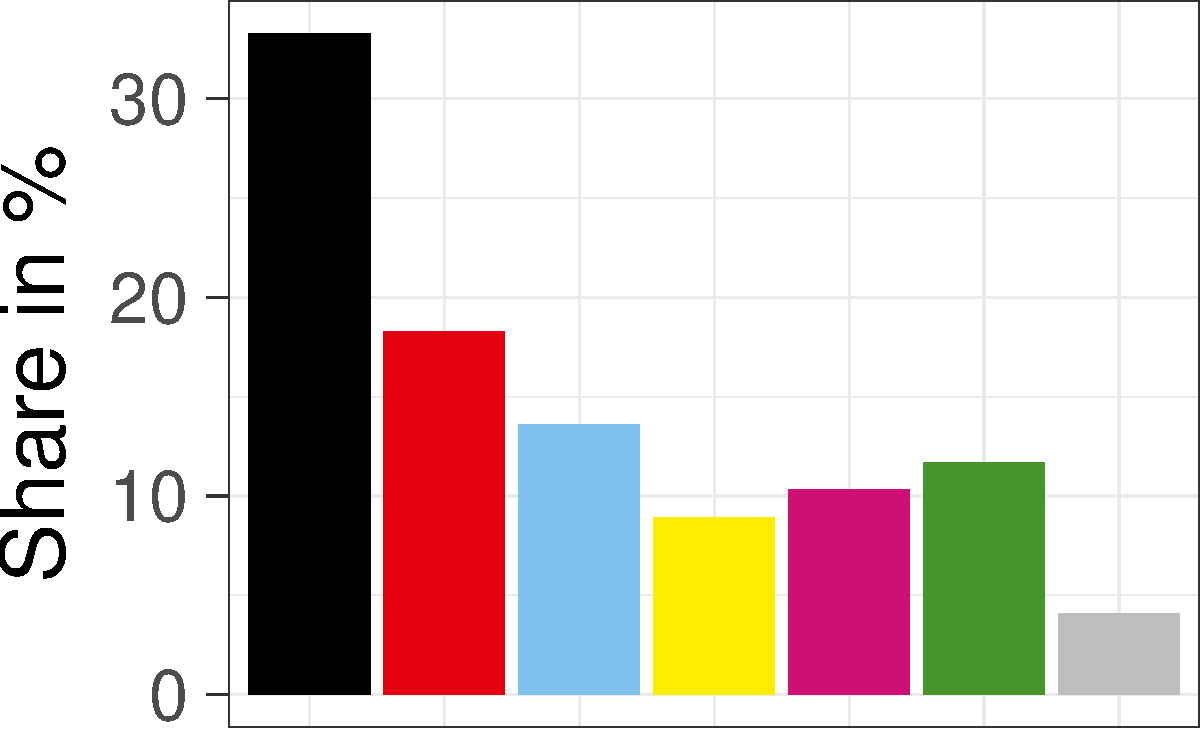
\includegraphics[height=4.75cm]{figures/motivation_survey}
  &
  \vspace{-4.5cm}
  \begin{itemize}
    \item \ldots is based on observed mean voter shares
    \item \ldots sets the focus on individual party achievements
    \item \ldots imparts sample uncertainty only insufficiently
  \end{itemize}
  \end{tabular}
  \\[2.5ex]
  % Example header
  {
  \setlength{\fboxrule}{3pt} % Border thickness
  \fcolorbox{koalawhitegray}{koalawhitegray2}{
  \begin{minipage}{0.9\textwidth}
  \vspace{2.5ex}
  \begin{center}\centering
  \bfBlue{Example} \\
  {\footnotesize \lightgray{Reporting on}} \darkgray{Union} {\footnotesize \lightgray{and}} \darkgray{FDP} {\footnotesize \lightgray{to jointly obtain a majority before the German federal election 2013}}
  \end{center}
  \vspace{2ex}
  \end{minipage}
  }
  }
  \end{column}

  % \hspace{-3.1ex}
  % \textcolor{LMUlightgray}{\vrule{}}
  % \hspace{3.1ex}
  
  \begin{column}{.475\textwidth}
  \colHeader{What do we propose?}
  Good reporting should:
  \vspace{2.5ex}
  \begin{itemize}
    \item \ldots impart findings in an easily graspable way
    \item \ldots prevent potential misunderstandings
    \item \ldots focus on the most relevant topics
  \end{itemize}
  \vspace{6.2ex}
  We aim at \textbf{shifting the focus} from \\[1.3ex]
  \begin{tabular}{clccl}
  \multirow{2}{*}[-0.95ex]{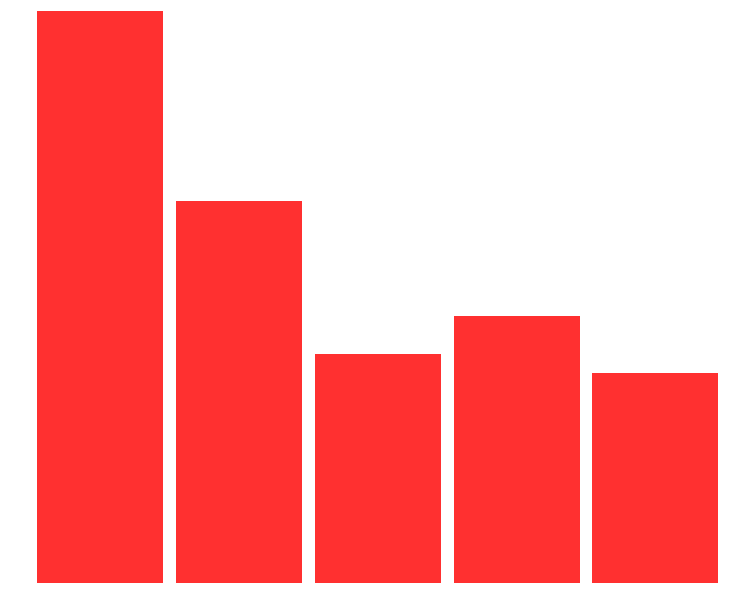
\includegraphics[height=3ex]{figures/motivation_pictoBar_col}} & 
  \darkgray{\footnotesize Incomprehensive} &
  \multirow{2}{*}{\ \ \darkgray{to} \ } &
  \multirow{2}{*}[-1ex]{
\includegraphics[height=3ex]{figures/motivation_pictoDens_col}} & 
  \darkgray{\footnotesize Uncertainty-based} \\
   & observed party shares & & & event probabilities \\
  \end{tabular}
  \end{column}

  \end{columns}
  
  % \noindent\hfil\textcolor{LMUlightgray}{\rule{0.93\textwidth}{.4pt}}\hfil
  % % \textcolor{LMUlightgray}{\hrule{}}
  % \vspace{3ex}
  
  % Lower columns with a specific example ----
  {
  \vspace{-4pt}
  \hspace{-24.34pt}
  \setlength{\fboxrule}{3pt} % Border thickness
  \fcolorbox{koalawhitegray}{koalawhitegray3}{
  \begin{minipage}{.96\textwidth}
  \vspace{3ex}
  \begin{columns}[t]

  \begin{column}{.29\textwidth}
  \darkgray{Last pre-election opinion poll:} \lightgray{\tiny Source: Forsa, 20.09.2013}
  \\[2.5ex]
  \begin{center}\centering
  % \scalebox{0.75} & {\footnotesize \lightgray{26\%}} & {\footnotesize \lightgray{10\%}} & \darkgray{5\%} & {\footnotesize \lightgray{9\%}} & {\footnotesize \lightgray{4\%}} & {\footnotesize \lightgray{6\%}} \\
  \bottomrule
  \end{tabular}
  % }
  \end{center}
  \vspace{1.5ex}
  \begin{center}\centering
  \darkgray{After redistribution} \lightgray{\footnotesize of party votes $<$5\% \\ (i.e. the minimum hurdle to pass into German parliament)} \\
  \darkgray{Union-FDP} \lightgray{\footnotesize jointly} \darkgray{obtain} \lightgray{\footnotesize exactly} \darkgray{50\%}.
  \end{center}
  \vspace{-3ex}
  \textcolor{koalablue}{$$ \underbrace{\resizebox{\hsize}{!}{ }}_{ } $$}
  \ \\ \vspace{-2ex}
  \begin{mdleftred}
  \begin{minipage}{\textwidth}
  \lightgray{\footnotesize Media headline:}
  \\
  \begin{center}\centering
  \vspace{-2ex}
  \darkgray{\textit{``Union-FDP loses its majority''}}
  \vspace{-.2ex}
  \end{center}
  \lightgray{\tiny Source: FAZ.net (2017). Umfrage zur Bundestagswahl: Schwarz-Gelb verliert \\[-2ex]
  die Mehrheit.http://archive.is/SuXVt. Accessed 26 April 2018.}
  \end{minipage}
  \end{mdleftred}
  \end{column}

  \begin{column}{.025\textwidth}
  \vspace{11ex}
  \huge{\blue{\ding{223}}}
  \end{column}

  \begin{column}{.26\textwidth}
  Flaws of this type of reporting:
  \vspace{1.5ex}
  \begin{itemize}
    \item \darkgray{Misleading conclusions are drawn} \\[0.2cm] \fnlightgray{A mean share of 50\% only means that it's} \fndarkgray{slightly more probable} \fnlightgray{that a majority is missed}
    \item \darkgray{Sample uncertainty is ignored} \\[0.2cm] \fnlightgray{E.g., with a mean voter share of 5\%, FDP will only enter the parliament with $\sim$50\%}
    \item \darkgray{Redistribution of votes is ignored} \\[0.2cm] \fnlightgray{FAZ.net bases the conclusion on the observed voter share and not on the redistributed 50\% share}
  \end{itemize}
  \end{column}

  \begin{column}{.025\textwidth}
  \vspace{11ex}
  \huge{\blue{\ding{223}}}
  \end{column}

  \begin{column}{.29\textwidth}
  Foundations of KOALA-based reporting:
  \vspace{1.5ex}
  \begin{itemize}
    \item \darkgray{Use event \textbf{probabilities}} \fnlightgray{instead of voter shares} \\[0.2cm] \fnlightgray{Probabilities comprise sample uncertainty in a natural way and are less at risk to be misinterpreted}
    \item \darkgray{Use \textbf{event} probabilities} \fnlightgray{instead of voter shares} \\[0.2cm] \fnlightgray{Focusing on the main events allows the reader to easily grasp the big picture}
  \end{itemize}
  \vspace{-1.7ex}
  \textcolor{koalablue}{$$ \underbrace{\resizebox{\hsize}{!}{ }}_{ } $$}
  \ \\ \vspace{-2ex}
  
  \begin{mdleftgreen}
  \begin{minipage}{\textwidth}
  \lightgray{\footnotesize KOALA headline:}
  \begin{center}\centering
  \darkgray{\textit{
  ``Union-FDP gains seat majority with 26\%, \ \ \\[0.1cm] \ \ FDP passes into parliament with 51\%$^*$''
  }}
  \end{center}
  \vspace{-0.7ex}
  \lightgray{\tiny ${}^*$ If the election was held today}
  \end{minipage}
  % }
  \end{mdleftgreen}
  \end{column}
  \end{columns}
  \end{minipage}
  }
  }

  \vspace{1ex}
\end{block}
\end{minipage}
\end{beamercolorbox}



% Begin main part -----------------------------------
\vspace{2ex}
\begin{columns}[T]

% empty space on left
\begin{column}{.016\textwidth}
\end{column}

\begin{column}{.484\textwidth}
\begin{beamercolorbox}[center,wd=\textwidth]{postercolumn}
\begin{minipage}[T]{.95\textwidth}  % tweaks the width, makes a new \textwidth
% \parbox[t][\columnheight]{\textwidth}{ % must be some better way to set the the height, width and textwidth simultaneously
% Since all columns are the same length, it is all nice and tidy.  You have to get the height empirically

% Main block 1 ---------------------------------------
\begin{block}{\footnotesize \circled{1} Probability estimation}
text
\end{block}


% Main block 2 -------------------------------------
\begin{block}{\footnotesize \circled{2} Visualization}
text
\end{block}



% Begin second column of main part -----------------
\end{minipage}
\end{beamercolorbox}
\end{column}

\begin{column}{.484\textwidth}
\begin{beamercolorbox}[center,wd=\textwidth]{postercolumn}
\begin{minipage}[T]{.95\textwidth}  % tweaks the width, makes a new \textwidth


% Implementation -----------------------------------
\begin{block}{\footnotesize \circled{3} Implementation}
\begin{center}\centering

\includegraphics[height=5ex]{figures/Koala_Logo_ohneSchrift}
\\[2ex]
Results for selected elections are presented on
\bfBlue{\texttt{\href{http://koala.stat.uni-muenchen.de}{koala.stat.uni-muenchen.de}}}
\end{center}
\vspace{2ex}
The implementation is based on several points:
\begin{itemize}
  \item Our approach is implemented in the R package \bfBlue{\texttt{coalitions}} 
  \item The website is shiny-based
  \item The website update approach is automated
  \item Automatic tweets are sent in the case of new results
  \item For sharing our results we automatically export them to Google Sheets
\end{itemize}

% Footer with software icons
\vspace{1ex}
\textcolor{LMUlightgray}{\hrule{}}
\vspace{1ex}
\begin{columns}[t]
  \begin{column}{.15\textwidth}
  \begin{center}\centering
  
\includegraphics[height=5ex]{figures/implementation_r}
  \end{center}
  \end{column}

  \hspace{-1.5ex}
  \textcolor{LMUlightgray}{\vrule{}}
  \hspace{1.5ex}

  \begin{column}{.15\textwidth}
  \begin{center}\centering
  \vspace{1ex}
  
\includegraphics[height=3ex]{figures/implementation_shiny}
  \end{center}
  \end{column}

  \hspace{-1.5ex}
  \textcolor{LMUlightgray}{\vrule{}}
  \hspace{1.5ex}

  \begin{column}{.15\textwidth}
  \begin{center}\centering
  
\includegraphics[height=5ex]{figures/hexSticker_icon}
  \end{center}
  \end{column}

  \hspace{-1.5ex}
  \textcolor{LMUlightgray}{\vrule{}}
  \hspace{1.5ex}

  \begin{column}{.15\textwidth}
  \begin{center}\centering
  
\includegraphics[height=5ex]{figures/implementation_sheets}
  \end{center}
  \end{column}

  \hspace{-1.5ex}
  \textcolor{LMUlightgray}{\vrule{}}
  \hspace{1.5ex}

  \begin{column}{.15\textwidth}
  \begin{center}\centering
  
\includegraphics[height=5ex]{figures/implementation_twitter}
  \end{center}
  \end{column}
\end{columns}
\end{block}

% Communication -----------------------------------
\begin{block}{\footnotesize \circled{4} Results communication}
text
\end{block}


% End main part ------------------------------------
\end{minipage}
\end{beamercolorbox}
\end{column}

% empty space on right
\begin{column}{.016\textwidth}
\end{column}

\end{columns}


% Literature ---------------------------------------
\vspace{2ex}
\begin{beamercolorbox}[center,wd=\textwidth]{postercolumn}
\begin{minipage}[T]{.95\textwidth}  % tweaks the width, makes a new \textwidth
\begin{block}{\footnotesize References}
{\footnotesize
Bender, A. and Bauer, A. (2018). coalitions: Coalition probabilities in multi-party democracies.
\textit{Journal of Open Source Software}, \textbf{3(23)}, 606,
\href{https://doi.org/10.21105/joss.00606}{\texttt{https://doi.org/10.21105/joss.00606}}. \\
Gelman, A. et al. (2013). \textit{Bayesian Data Analysis, 3rd edition}. Boca Raton, FL: CRC press.
}
\end{block}
\end{minipage}
\end{beamercolorbox}

% End page -----------------------------------------
\end{column} % 1 Spalte, die die ganze Seite einnimmt
\end{columns}
\end{frame}
\end{document}
  
  
  %%%%%%%%%%%%%%%%%%%%%%%%%%%%%%%%%%%%%%%%%%%%%%%%%%%%%%%%%%%%%%%%%%%%%%%%%%%%%%%%%%%%%%%%%%%%%%%%%%%%
    %%% Local Variables: 
    %%% mode: latex
  %%% TeX-PDF-mode: t
  %%% End:
    